\appendix
\section{Application}
	
	We use this additional section to address the details of Example~\ref{ex:example1}.
	
\begin{example}[Detailed analysis of Example~\ref{ex:example1}]
	Let the base types $\intk$ and $\boolk$ represent integer and Boolean values, $\ell$ and $m$ denote labels for the internal and external choices on the branches, and consider the types:
	\[
	S\triangleq \mu x. (\oplus\{\ell\colon !\,\intk; \&\{\ell\colon x, m\colon \skipk \} , m\colon !\, \boolk; \&\{\ell\colon x, m\colon \skipk \} \}); \mu x. (\&\{\ell\colon\skipk, m\colon ?\,\boolk; x \})
	\]
	\[
	T\triangleq \mu x. (\oplus\{\ell\colon !\,\intk , m\colon !\, \boolk\}; \&\{\ell\colon x, m\colon \mu y. (\&\{\ell\colon\skipk, m\colon ?\,\boolk; y \})\})
	\]
	$S$ and $T$ can be represented as PA graphs as depicted on Figure~\ref{fig:PAgraphsST}.
	
	\begin{figure}[h!]
		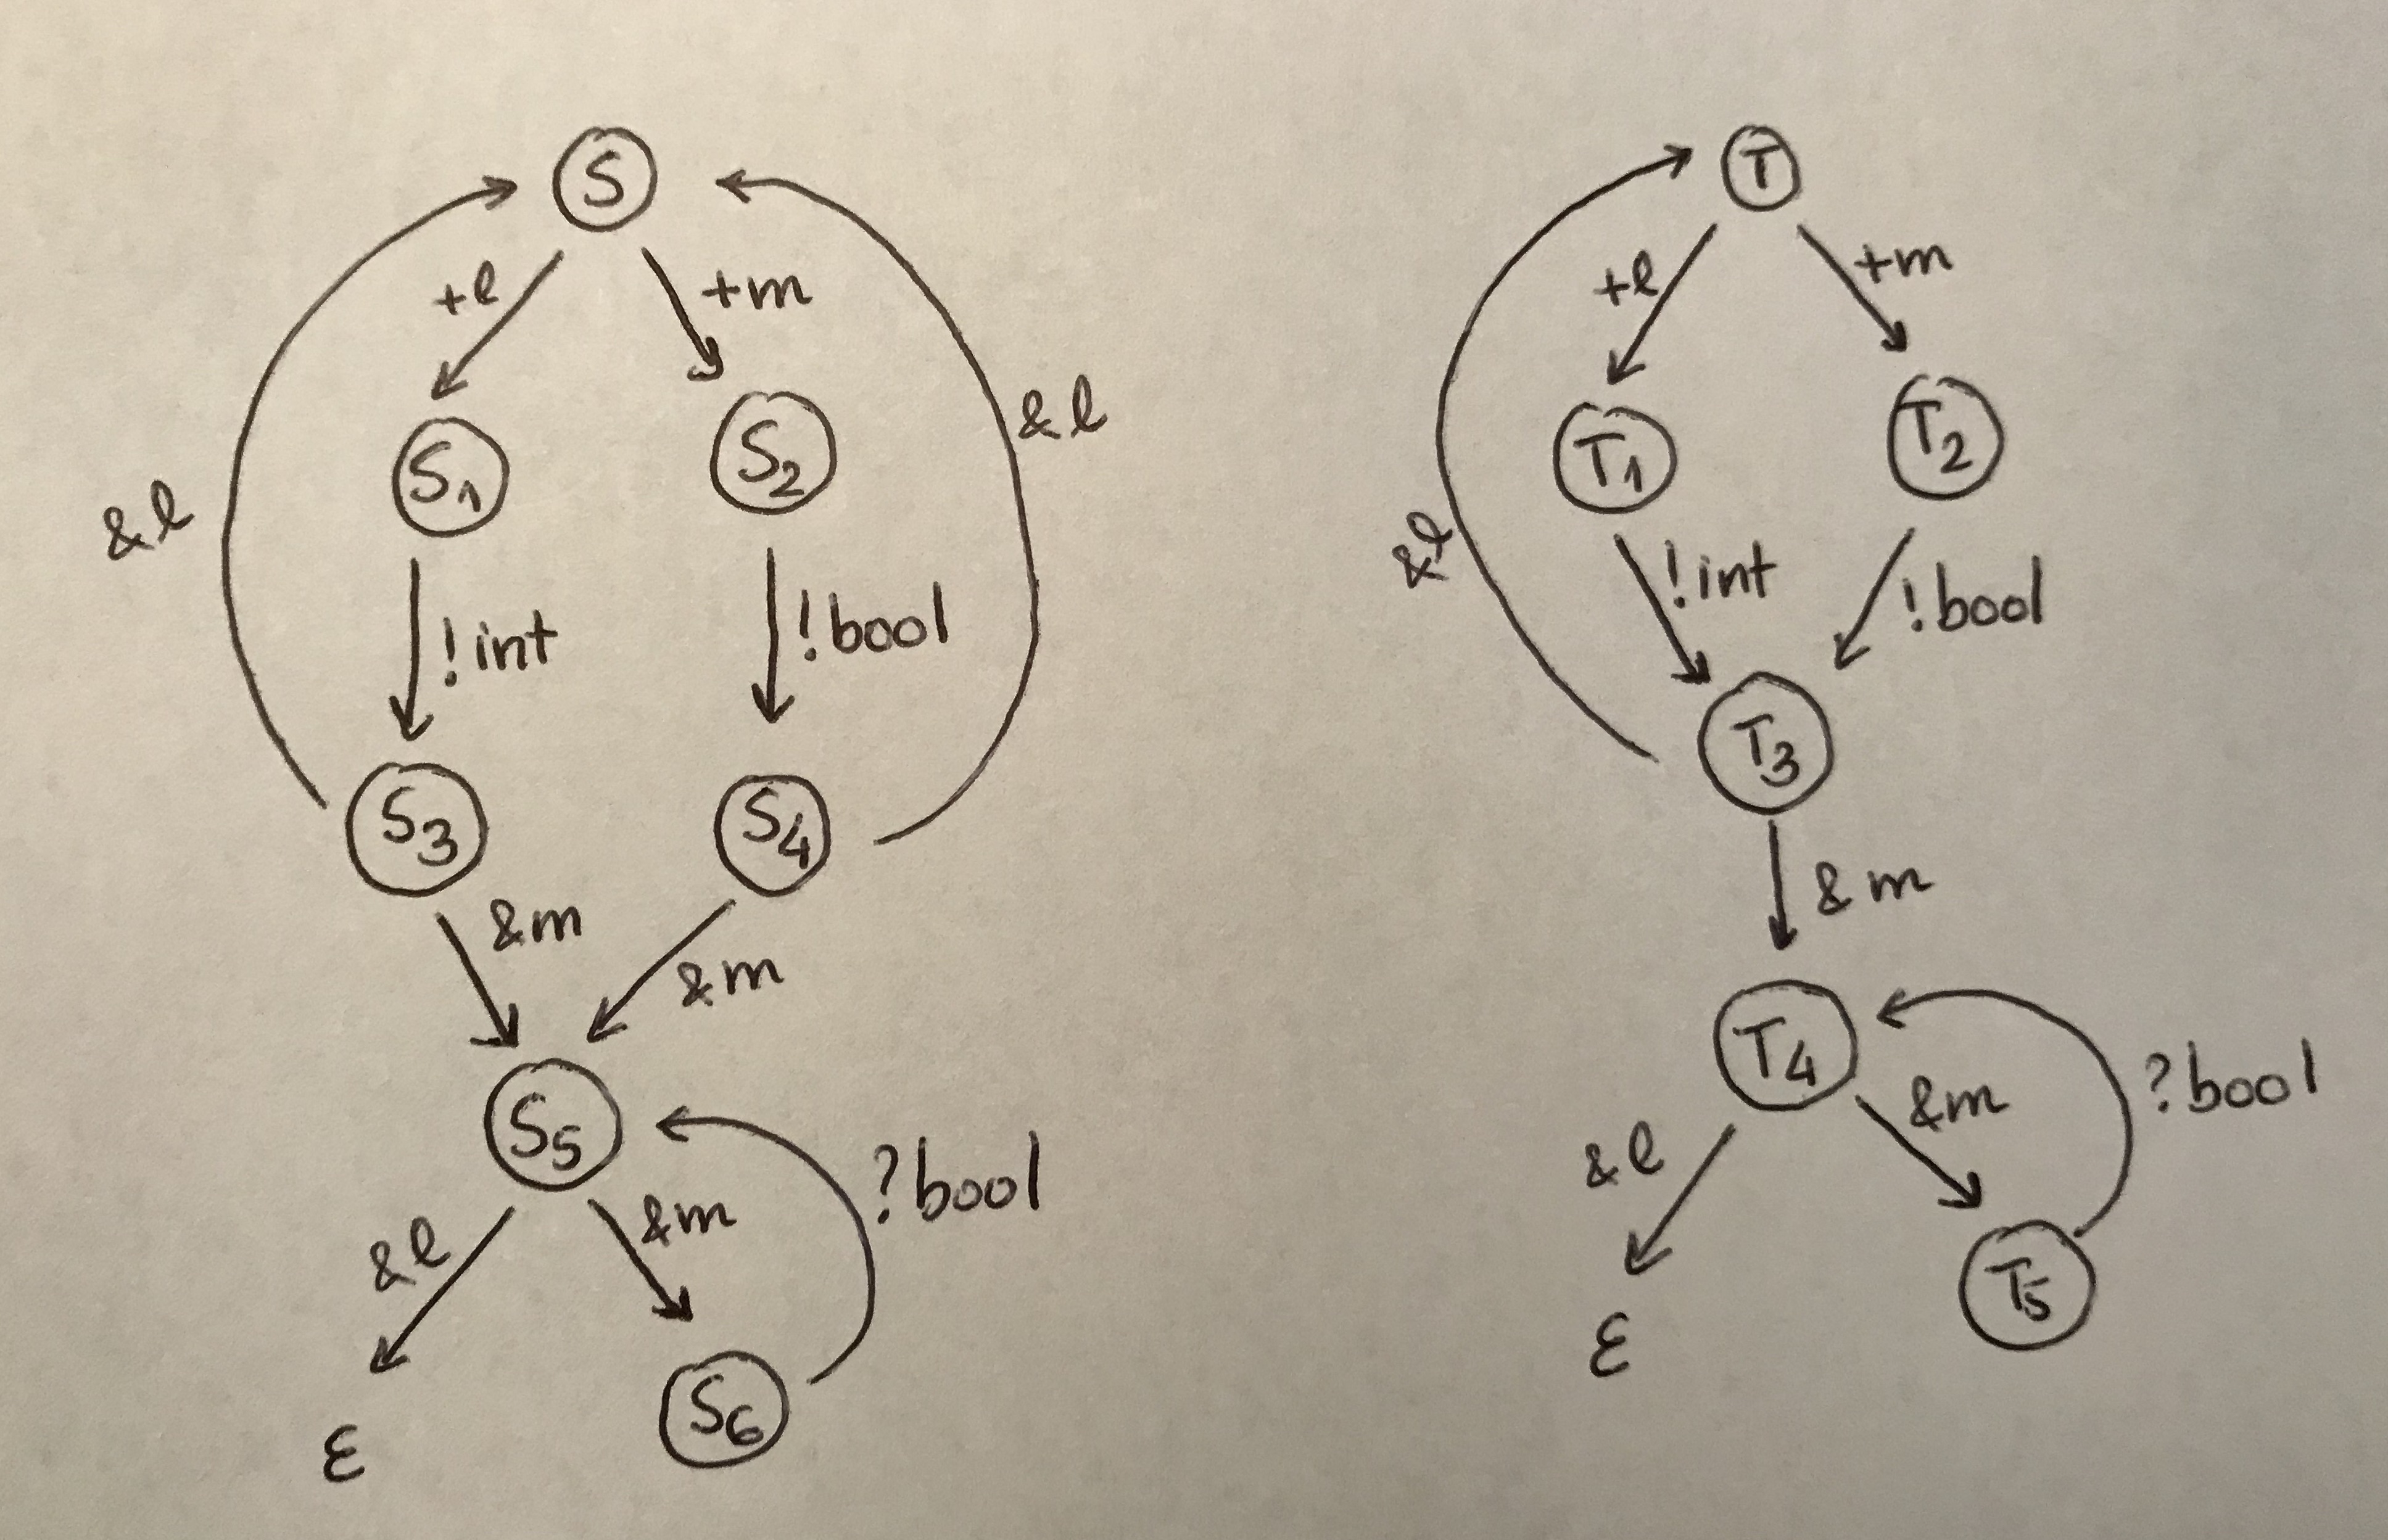
\includegraphics[width=\columnwidth]{PAgraphsST.jpg}
		\caption{Process algebra graphs for $S$ and $T$.}
			\label{fig:PAgraphsST}
	\end{figure}
	The algorithm we propose in this work derives the expansion tree for $S\sim T$ as a sequence of nodes. The nodes in this expansion tree can be labeled with a trace of the nodes that lie ahead, based on the syntactical structure of $S$ and $T$. We get the following sequence of labeled nodes in the expansion tree for $S\sim T$:\\\\
\begin{tikzcd}[cells={nodes={draw=black}}, column sep=large]
  \enspace (S,T) \enspace \ar[r,"expand"]
& \enspace  (S_1S_3S_5,T_1T_3), (S_2S_4S_5, T_2T_3) \enspace \ar[r,"expand"]
& \enspace  (S_3S_5,T_3), (S_4S_5, T_3) \enspace  
\end{tikzcd} 
$\xrightarrow{\text{expand}}$\\\\
\begin{tikzcd}[cells={nodes={draw=black}}, column sep=large]
& \enspace(SS_5,T),(SS_5,T),(S_5,T_4),(S_5,T_4)  \enspace\ar[r,dashed,"bpa1"]
&\enspace (S_5,\varepsilon),(S_5,T_4) \enspace 
\end{tikzcd} 
$\xrightarrow{\text{expand}}$ \\\\
\begin{tikzcd}[cells={nodes={draw=black}}, column sep=large]
&\enspace (S_6S_5,T_5T_4), (\varepsilon,\varepsilon) \enspace \ar[r,dashed,"reflex"] 
&\enspace (S_6S_5,T_5T_4)\enspace \ar[r,"expand"]
& \enspace(S_5,T_4)\enspace \ar[r,dashed,"bpa1"]
&\emptyset\\
\end{tikzcd}

	The process alternates between simplification and expansion operations, denoted by dashed and solid arrows, respectively. Having reached an empty node, we conclude that $S\sim T$.\\\smallskip
	
	Now consider the types:
	\[ R \triangleq \mu x.\&\{\ell\colon ?\,\boolk;x, m\colon ?\,\intk;x;x \} \text{ and }  U \triangleq \mu x.\&\{\ell\colon ?\,\boolk, m\colon ?\,\intk;x;x\} \enspace .\]
	
	$R$ and $U$ are represented as PA graphs as shown in Figure~\ref{fig:PAgraphsRU}.
	
	\begin{figure}[h!]
	\centering
		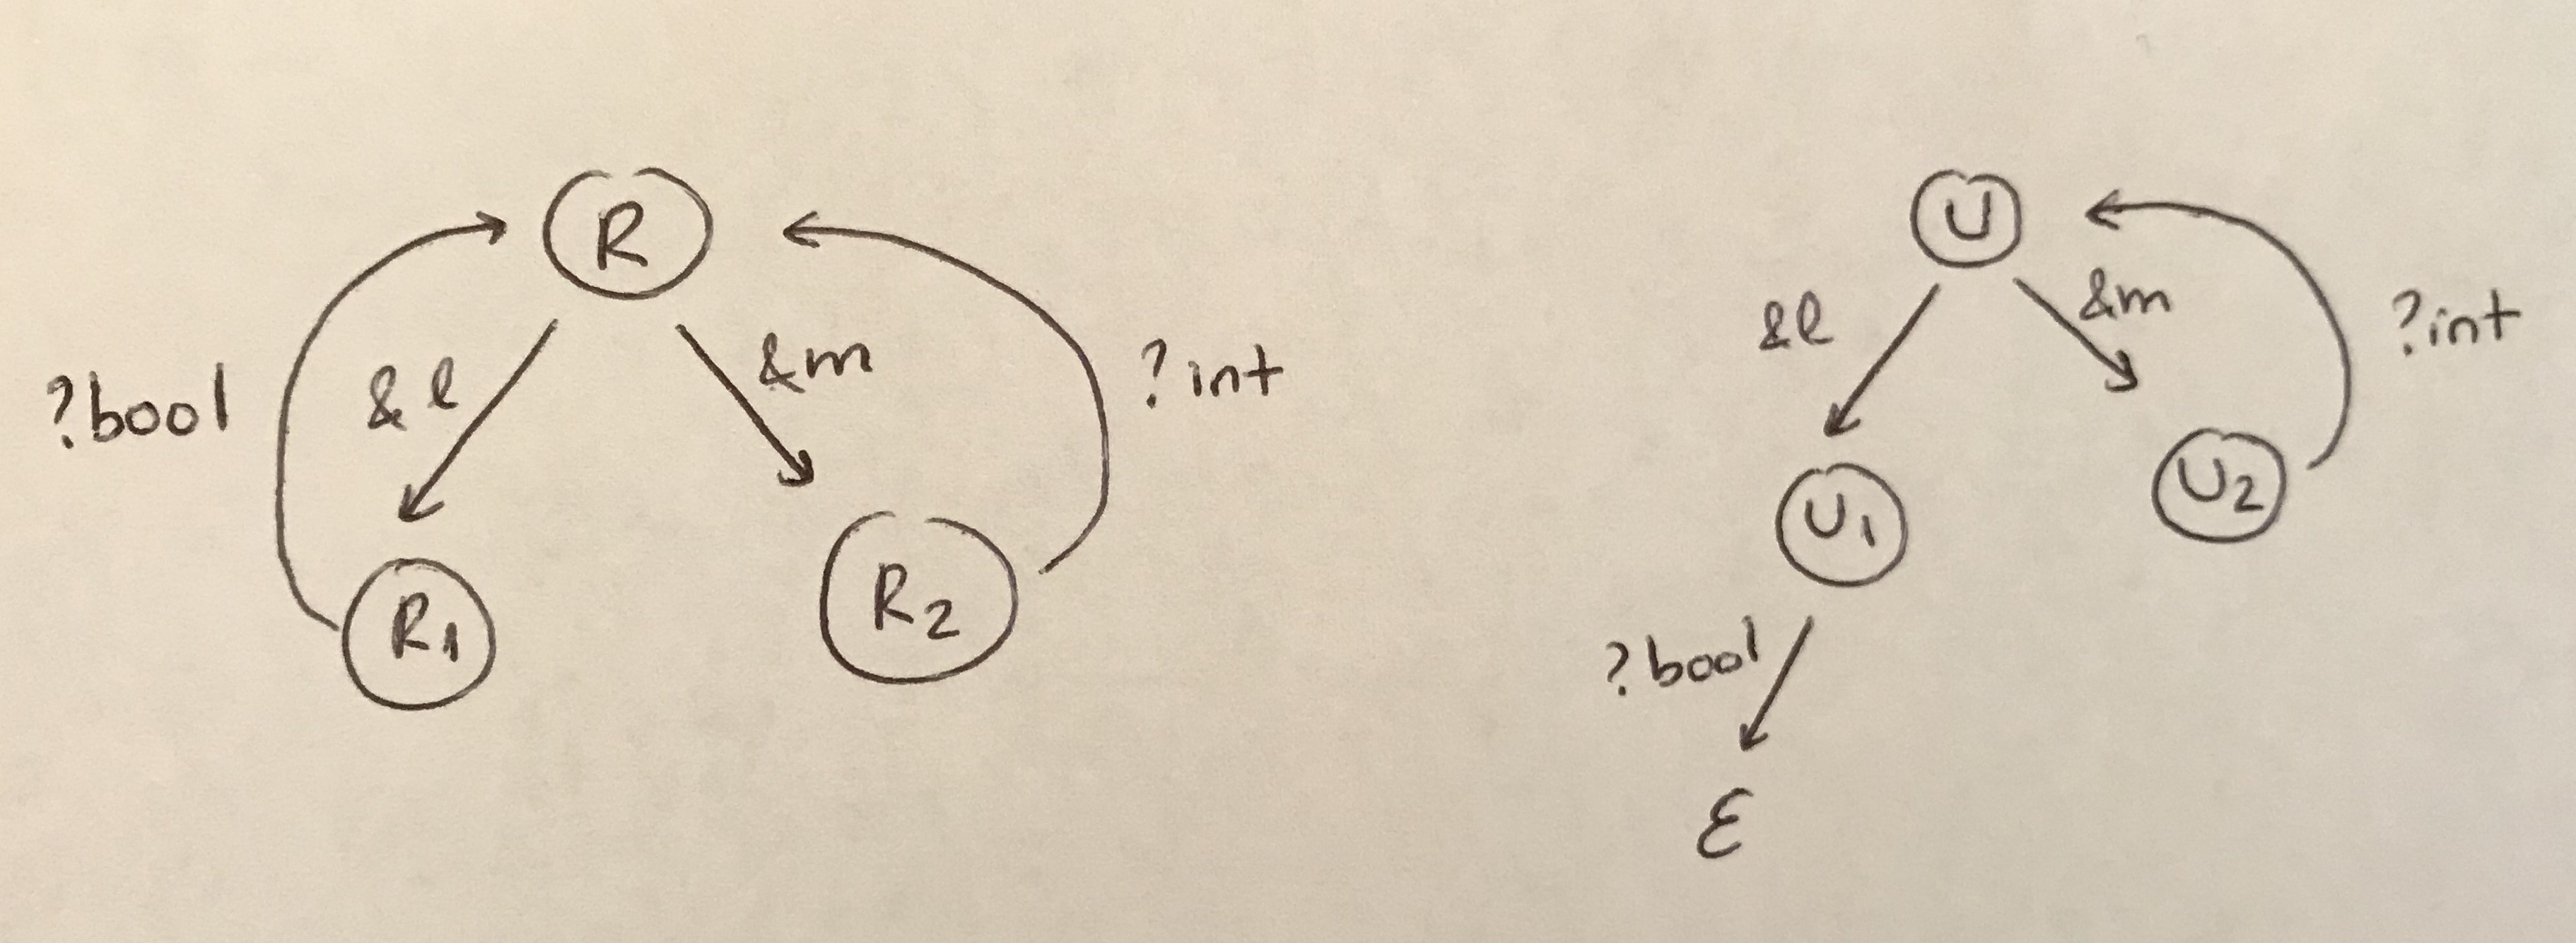
\includegraphics[width=14cm]{PAgraphsRU.jpg}
		\caption{Process algebra graphs for $R$ and $U$.}
		\label{fig:PAgraphsRU}
	\end{figure}
	Using the porposed algorithm, we get the following expansion list build upon the syntactical structure of $R$ and $U$ and their representations as PA graphs:\\\\
\begin{tikzcd}[cells={nodes={draw=black}}, column sep=large]
  (R,U) \ar[r,"expand"]
& (R_1 R,U_1), (R_2 R R, U_2 U U) \ar[r,"expand"]
& (R,\varepsilon), (RR, UU) \ar[r,dashed,"bpa1"] 
& (R,\varepsilon), (U,\varepsilon) 
\end{tikzcd} 
\enspace  $\times$\\\\
We notice that the last step results from applying BPA1 rule~\cite{janvcar1999techniques} to $(RR,UU)$ knowing that $(R,U)$ is an ancestor node, which leads to the pairs $(R,\varepsilon)$ and $(U,\varepsilon)$. As we then fail to obtain new derived nodes, we decide the type equivalence negatively and conclude that $R\not\sim U$.
	\hfill $\triangle$
\end{example}
